\section{Methodology}
\label{sec:methodology}

Figure~\ref{fig:method-overview} summarizes the methodology. We first evaluate the learned policy inside its source RLTabucol framework against random-policy and Pure Tabucol controls. Because this comparison shows useful but non-uniform policy effects, the actor-only diagnostic then isolates the policy's standalone behavior and examines whether the policy--Tabucol interaction is a plausible source of the remaining failures. This diagnosis
motivates RLACO, a cross-framework transfer framework that reuses the frozen
policy in ACO through soft pheromone injection. Finally, we use the learned
soft-prior RLACO configuration to initialize a downstream Tabucol solver,
testing whether RLACO$\rightarrow$Tabucol can convert the transferred guidance
into stronger final graph-coloring optimization. 

\begin{figure*}[t]
\centering
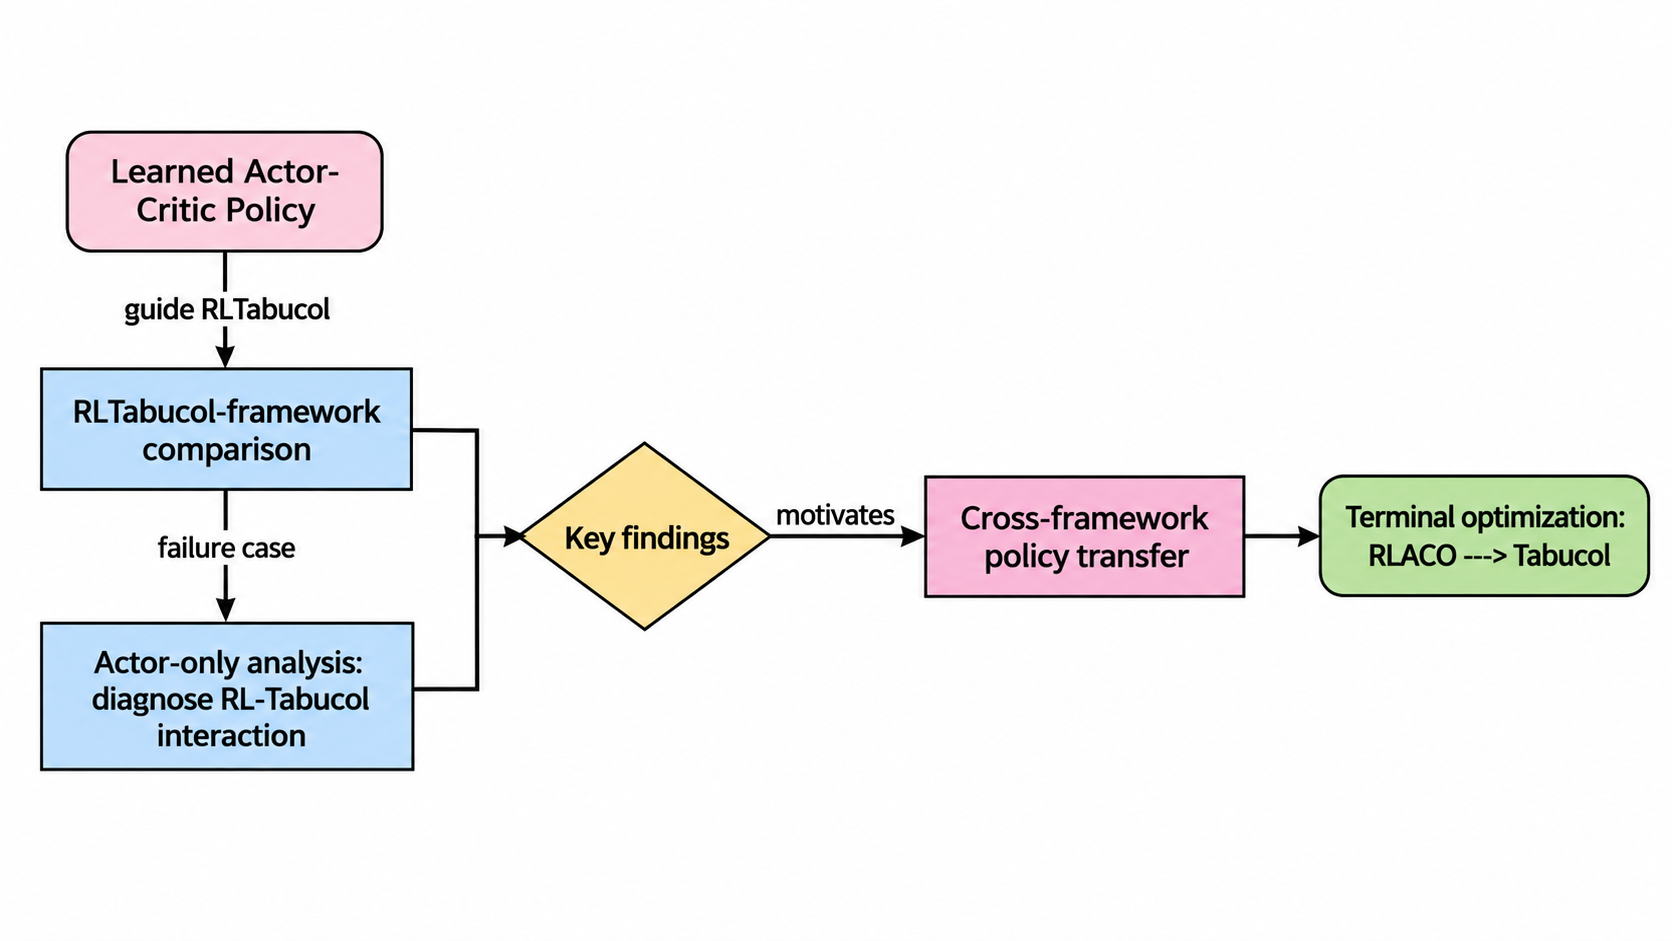
\includegraphics[width=\linewidth]{../figures/method_overview.png}
\caption{Overview of the methodology. A single actor--critic policy is trained in the source RLTabucol setting, frozen, and then evaluated through source-framework comparison, actor-only diagnosis, cross-framework transfer to ACO, and terminal RLACO$\rightarrow$Tabucol optimization.}
\label{fig:method-overview}
\end{figure*}

\subsection{Learned Actor-Critic policy}
\label{ssec:policy}

The shared learned policy selects vertex--color recoloring actions. We model each RL phase as a finite-horizon Markov decision process consisting of \(I\) sequential recoloring steps. At step $t$, the state contains the graph $G=(V,E)$, the color budget $k$, and the current coloring $c_t$. An action is a vertex--color pair $a_t=(v_t,q_t)$ specifying the vertex to recolor and its target color. The immediate reward at RL step $t$ is the reduction in the number of
conflicting edges caused by the recoloring:
\begin{equation}
r_t^{\mathrm{imm}}
=
f(c_{t-1})-f(c_t),
\label{eq:immediate-reward}
\end{equation}
where $f(c)$ denotes the number of conflicting edges in coloring $c$.
Thus, a positive reward indicates conflict reduction, zero indicates no
change, and a negative reward indicates an increase in conflicts. After the final RL step, the resulting coloring $c_I$ is passed to
Tabucol. If $c^{\mathrm{ret}}$ is the coloring returned by Tabucol, the
downstream reward is
\begin{equation}
r_{\mathrm{Tabu}}
=
f(c_I)-f(c^{\mathrm{ret}}).
\label{eq:tabu-reward}
\end{equation}

The reward used for the RL transition is therefore
\begin{equation}
r_t
=
r_t^{\mathrm{imm}}
+
\mathbb{I}[t=I]\,r_{\mathrm{Tabu}},
\label{eq:total-reward}
\end{equation}
where $\mathbb{I}[t=I]$ is one only for the final RL transition and zero
otherwise. With $I=300$, the first $299$ transitions receive only the
immediate conflict-reduction reward, while the $300$th transition receives
both the immediate reward and the downstream Tabucol reward. Therefore, this  reward is intended to encourage the policy not only to reduce conflicts during the RL phase, but also to favor handoff states that allow Tabucol to make further progress.


The policy is implemented as an actor--critic architecture. The actor network factorizes the joint action distribution into a vertex-selection distribution and a conditional color-selection distribution:
\begin{equation}
  \pi_{\theta,\phi}((v,q)\mid s)
  =
  \pi^{\mathrm{v}}_\theta(v\mid s)\,
  \pi^{\mathrm{c}}_\phi(q\mid s,v).
  \label{eq:rl_policy_factorisation}
\end{equation}
The vertex-selection head $\pi^{\mathrm{v}}_\theta$ is a two-layer multilayer perceptron ($3\!\to\!16\!\to\!1$ with ReLU) applied independently to each vertex, followed by a softmax over vertices. It uses three vertex-level features: degree, conflicting-edge count, and number of distinct neighbor colors. The color-selection head $\pi^{\mathrm{c}}_\phi$ is a separate two-layer MLP with the same width, applied to each vertex--color pair and followed by a softmax over colors. It uses three color-level features: number of neighbors assigned the candidate color, color-class size, and total vertex count. Because the same MLP is applied independently to every vertex or vertex--color pair, changing the graph size or color budget changes only the number of evaluations, not the actor's parameters, the actor can be evaluated on different graph sizes and color budgets without changing its parameterization.

The critic uses the same feature-processing structure without the actor softmax layers and appends a linear layer over the flattened $n\times k$ representation to estimate the scalar state value $V_\psi(s)$. This value is used to compute advantage estimates for Proximal Policy Optimization (PPO)~\cite{schulman2017ppo}; PPO updates both actor and critic parameters using the standard clipped surrogate objective. We train a single source policy on Erd\H{o}s--R\'enyi
$G(n{=}250,p{=}0.5)$ graphs with $k{=}24$ for $50$ training epochs; this fixed training setting provides
one common source policy for all subsequent experiments. The same policy
is reused without fine-tuning so that differences across the source, transfer,
and terminal experiments reflect how the policy is used in each framework,
rather than differences caused by retraining or selecting different policies. Detailed PPO and training parameters are reported in Appendix~\ref{app:experimental-details}.

\subsection{RLTabucol source framework}
\label{ssec:rltabucol}

We implement RLTabucol by interleaving the learned policy with Tabucol local search within an episodic loop~\cite{cai2019rlho,frijters2023rltabucol}. Each run starts from a random $k$-coloring. 

Within each episode, the actor performs $I$ sequential recoloring steps, producing an intermediate coloring that is then passed to Tabucol. Tabucol is a single-solution local search that iteratively selects the best admissible vertex recoloring, subject to a tabu list that prevents recently reversed moves. Within RLTabucol, Tabucol performs at most $T$ single-vertex recoloring iterations and returns both a coloring and the reward in Eq.~\eqref{eq:tabu-reward}. The detailed Tabucol procedure is given in Algorithm~\ref{alg:tabucol} in Appendix~\ref{app:experimental-details}.

The returned coloring becomes the starting state of the next episode. With probability $\beta$, Tabucol returns its current coloring; with probability $1-\beta$, it returns the best coloring found during Tabucol phase. The best coloring is therefore retained most of the time, while occasionally
returning the current coloring allows the next RL episode to continue from a
different state rather than always from the local best.  RLTabucol therefore follows one continuing sequence of RL and Tabucol updates rather than restarting independently at every episode. Algorithm~\ref{alg:rltabucol} summarizes the complete pipeline. During training, the collected trajectories are used for PPO updates; during testing, the actor remains fixed.

\begin{algorithm}[t]
\caption{The RLTabucol pipeline}
\label{alg:rltabucol}
\begin{algorithmic}[1]
\State \textbf{Input:} $G$, $k$, actor $\pi_{\theta,\phi}$, steps $I$,
Tabucol iters $T$, prob.\ $\beta$, budget $\mathcal{B}$
\State $c\leftarrow$ random $k$-coloring;\quad $c^\star\leftarrow c$
\While{$\mathcal{B}$ not exhausted}
  \For{$t=0,\dots,I-1$}
    \State $(v,q)\sim\pi_{\theta,\phi}(\cdot\mid(G,k,c))$;\quad $c\leftarrow c[v\mapsto q]$
    \If{$f(c)<f(c^\star)$} \State $c^\star\leftarrow c$ \EndIf
    \If{$f(c^\star)=0$} \State \Return $c^\star$ \EndIf
  \EndFor
  \State $c\leftarrow\textsc{Tabucol}(G,k,c,T,\beta)$
  \If{$f(c)<f(c^\star)$} \State $c^\star\leftarrow c$ \EndIf
  \If{$f(c^\star)=0$} \State \Return $c^\star$ \EndIf
\EndWhile
\State \Return $c^\star$
\end{algorithmic}
\end{algorithm}

Two baselines are used to evaluate RLTabucol. RLTabucol$_0$ replaces the trained actor with a uniform random policy over the same vertex--color action space while keeping the episodic RL--Tabucol structure unchanged; it tests whether the learned actor contributes useful guidance beyond random recoloring. Pure Tabucol uses the same Tabucol implementation and tabu settings as a standalone solver, without any RL guidance, providing a direct baseline for evaluating whether the RLTabucol framework improves over conventional Tabucol and becomes a stronger optimizer. Run counts, time limits, tested color budgets, and evaluation metrics are specified in Section~\ref{ssec:exp-settings}.

\subsection{Actor-only analysis}
\label{ssec:actor-only}

To further diagnose the inconsistent results and investigate the behavior of actor. We design and implement the actor-only diagnostic, which separates the policy's standalone conflict-reduction capability from the downstream repair supplied by Tabucol. Tabucol is disabled while the frozen actor performs the same $I$ recoloring steps, and the conflict trajectory and running-best value are recorded. Comparing this behavior with the full RLTabucol trajectory shows how far the actor can reduce conflicts by itself, how much additional repair is supplied by Tabucol, and whether the remaining difficulty is consistent with the interaction between the two stages rather than the complete failure of either component in isolation. The tested failure case and evaluation protocol are specified in Section~\ref{ssec:exp-settings}.

\subsection{Cross-framework transfer to ACO via soft pheromone injection}
\label{ssec:rlaco}

To test whether the learned policy remains useful when its guidance is consumed by a structurally different search process, we introduce RLACO, which transfers the same policy from the Tabucol-based source framework to ACO through soft pheromone injection. In RLACO, the actor's per-vertex color-selection distribution is mapped to
the initial pheromone matrix, thereby biasing the color choices of the ants.
Each ant then constructs a complete coloring from scratch under this soft
policy guidance. Thus, the transferred information is the policy's learned
color preference rather than a prescribed coloring, allowing the same frozen policy to guide multiple ACO constructions without retraining.

The ACO component follows a MAX--MIN ant system~\cite{stutzle2000maxmin} with pheromone clipping, elite reinforcement, and a pseudo-random-proportional construction rule. Each ant constructs a complete coloring by visiting vertices one by one and selecting colors from the combination of pheromone and heuristic information. The detailed ACO procedure is given in Algorithm~\ref{alg:aco} in Appendix~\ref{app:experimental-details}.

The key interface is soft pheromone injection. Given the current state $s$, the actor's color-selection head produces
$P(v,q)=\pi^{\mathrm{c}}_\phi(q\mid s,v)$, with
$\sum_{q=1}^{k}P(v,q)=1$, representing the preference for assigning color $q$ to vertex $v$. At the end of each RL phase, before the corresponding ACO call, the pheromone matrix is reset to the uniform base level $\tau_0$ and the policy distribution is injected as
\begin{equation}
  \tau(v,q)
  \leftarrow
  \tau_0 +
  \bigl(\min(\tau_{\max},\, \sigma\tau_0) - \tau_0\bigr)\,
  P(v,q),
  \label{eq:soft}
\end{equation}
where $\sigma>1$ is the injection strength. The resulting pheromone values are clipped to $[\tau_{\min},\tau_{\max}]$. The actor provides a soft pheromone prior rather than a deterministic
coloring: each ant still constructs a complete coloring from scratch under
the biased pheromone. The coloring produced by the preceding RL phase is
retained separately as the initial ACO incumbent, while each ant still constructs a coloring from scratch under the biased
pheromone. Standard ACO evaporation and elite reinforcement then update
pheromone during the construction process.
Thus, the RL phase influences ACO through both the soft
pheromone bias and the initial incumbent. Algorithm~\ref{alg:rlaco} summarizes the transfer pipeline.

\begin{algorithm}[t]
\caption{The RLACO pipeline}
\label{alg:rlaco}
\begin{algorithmic}[1]
\State \textbf{Input:} $G$, $k$, actor $\pi_{\theta,\phi}$, steps $I$,
ACO iters $T_{\mathrm{ACO}}$, ants $m$, budget $B$
\State \textbf{Params:} $\tau_0,\tau_{\min},\tau_{\max},\sigma$
\State $c\leftarrow$ random $k$-coloring;\quad $c^\star\leftarrow c$
\While{elapsed $<B$}
  \For{$t=0,\dots,I-1$}
    \State $(v,q)\sim\pi_{\theta,\phi}(\cdot\mid s(c))$;\quad $c\leftarrow c[v\mapsto q]$
    \If{$f(c)<f(c^\star)$} \State $c^\star\leftarrow c$ \EndIf
  \EndFor
  \State $P(v,q)\leftarrow\pi^{\mathrm{c}}_\phi(q\mid s(c),v)$
  \State $\tau\leftarrow\textsc{SoftInject}(P,\tau_0,\tau_{\min},\tau_{\max},\sigma)$
  \State $c\leftarrow\textsc{ACO}(G,k,c,\tau,m,T_{\mathrm{ACO}})$
  \If{$f(c)<f(c^\star)$} \State $c^\star\leftarrow c$ \EndIf
  \If{$f(c^\star)=0$} \State \Return $c^\star$ \EndIf
\EndWhile
\State \Return $c^\star$
\end{algorithmic}
\end{algorithm}

To evaluate the transferred guidance, we compare RLACO$_{\rm soft}$ with three reference configurations: Pure ACO, the random-policy transfer reference RLACO$0$, and the structured conflict-prior configuration RLACO${\rm config}$.  RLACO$_0$ replaces the trained actor with a random policy while preserving the same RL-step and ACO structure. Since the random policy has no learned per-vertex distribution, its realized random-policy coloring is used to bias pheromone toward the vertex--color assignments present in that coloring; RLACO$_0$ is therefore a random-policy transfer reference rather than a perfectly matched soft-prior ablation. Pure ACO removes the RL phase and runs the same ACO continuously without external policy guidance; its pheromone state is retained throughout the run rather than reinitialized between successive ACO calls. RLACO$_{\rm config}$ retains the trained RL phase and the soft-injection mechanism but replaces the learned distribution with a structured conflict-based pheromone prior,
Let $H_v(s,q)$ denote the number of neighbors of vertex $v$ assigned
color $q$ in the complete post-RL coloring represented by state $s$.
The structured conflict-based pheromone prior is defined as
\begin{equation}
 P_{\mathrm{conf}}(v,q)
 =
 \frac{(1+H_v(s,q))^{-1}}
 {\sum_{r=1}^{k}(1+H_v(s,r))^{-1}},
 \label{eq:conf-prior}
\end{equation}
which assigns higher prior probability to colors that currently appear
less frequently among the neighbors of $v$. This baseline replaces the
learned color-selection distribution with a state-dependent structured
conflict-based prior while keeping the trained RL phase and the same
soft-injection pipeline unchanged. ACO local-search post-processing is disabled in RLACO, RLACO$_0$, RLACO$_{\rm config}$, and Pure ACO. This isolates transfer through the ACO construction process: adding local repair at this stage would mix the quality of the transferred guidance with the effect of a downstream local solver. The terminal experiment in Section~\ref{ssec:terminal-method} evaluates that complete optimization question separately.

To examine how the transferred guidance is used inside RLACO, we record the conflict count at three checkpoints in each episode: before the RL phase ($f_e^{\mathrm{start}}$), after the RL phase ($f_e^{\mathrm{RL}}$), and after ACO ($f_e^{\mathrm{ACO}}$). The positive conflict reduction attributed descriptively to each phase is
\begin{align}
  \Delta_e^{\mathrm{RL}}
  &=
  \bigl[f_e^{\mathrm{start}} - f_e^{\mathrm{RL}}\bigr]_+,
  &
  \Delta_e^{\mathrm{ACO}}
  &=
  \bigl[f_e^{\mathrm{RL}} - f_e^{\mathrm{ACO}}\bigr]_+,
\end{align}
where $[x]_+=\max(x,0)$ assigns zero positive reduction to a phase that increases conflicts. Aggregating over episodes gives $S_{\mathrm{RL}}$ and $S_{\mathrm{ACO}}$, with
\begin{equation}
  \mathrm{share}^{\mathrm{RL}}
  =
  \frac{S_{\mathrm{RL}}}
       {S_{\mathrm{RL}}+S_{\mathrm{ACO}}},
  \qquad
  \mathrm{share}^{\mathrm{ACO}}
  = 1 - \mathrm{share}^{\mathrm{RL}}.
  \label{eq:phase-share}
\end{equation}
Because ACO acts on the state produced by the preceding RL phase, these shares are descriptive rather than causal. They distinguish whether positive conflict reduction is recorded mainly during the RL phase or during the subsequent ACO construction phase.

\subsection{RLACO$\rightarrow$Tabucol terminal optimization}
\label{ssec:terminal-method}

The terminal RLACO$\rightarrow$Tabucol experiment tests whether the best coloring found by RLACO can provide a stronger starting point for Tabucol and thereby improve final graph-coloring performance to achieve the goal of optimization. We use the soft-injection RLACO configuration to construct an initialization, then pass its best coloring to downstream Tabucol run using the same Tabucol implementation as the Pure Tabucol baseline and no additional RL phase. Thus, We proposed a framework called RLACO$\rightarrow$Tabucol.
